\documentclass{article}

% Language setting
% Replace `english' with e.g. `spanish' to change the document language
\usepackage[english]{babel}

% Set page size and margins
% Replace `letterpaper' with `a4paper' for UK/EU standard size
\usepackage[letterpaper,top=2cm,bottom=2cm,left=3cm,right=3cm,marginparwidth=1.75cm]{geometry}

% Useful packages
\usepackage{amsmath}
\usepackage{graphicx}
\usepackage[colorlinks=true, allcolors=blue]{hyperref}

\title{PS6_Thomasson}
\author{Campbell Thomasson}

\begin{document}
\maketitle

\section{PS6}

I am a huge NBA buff, so I brought in the daily-updated table of NBA Draft Lottery odds for teams currently out of the NBA Playoff picture. 

My first plot is a distribution of the odds of each current lottery team to receive the 1st pick in the draft:

\begin{figure}
    \centering
    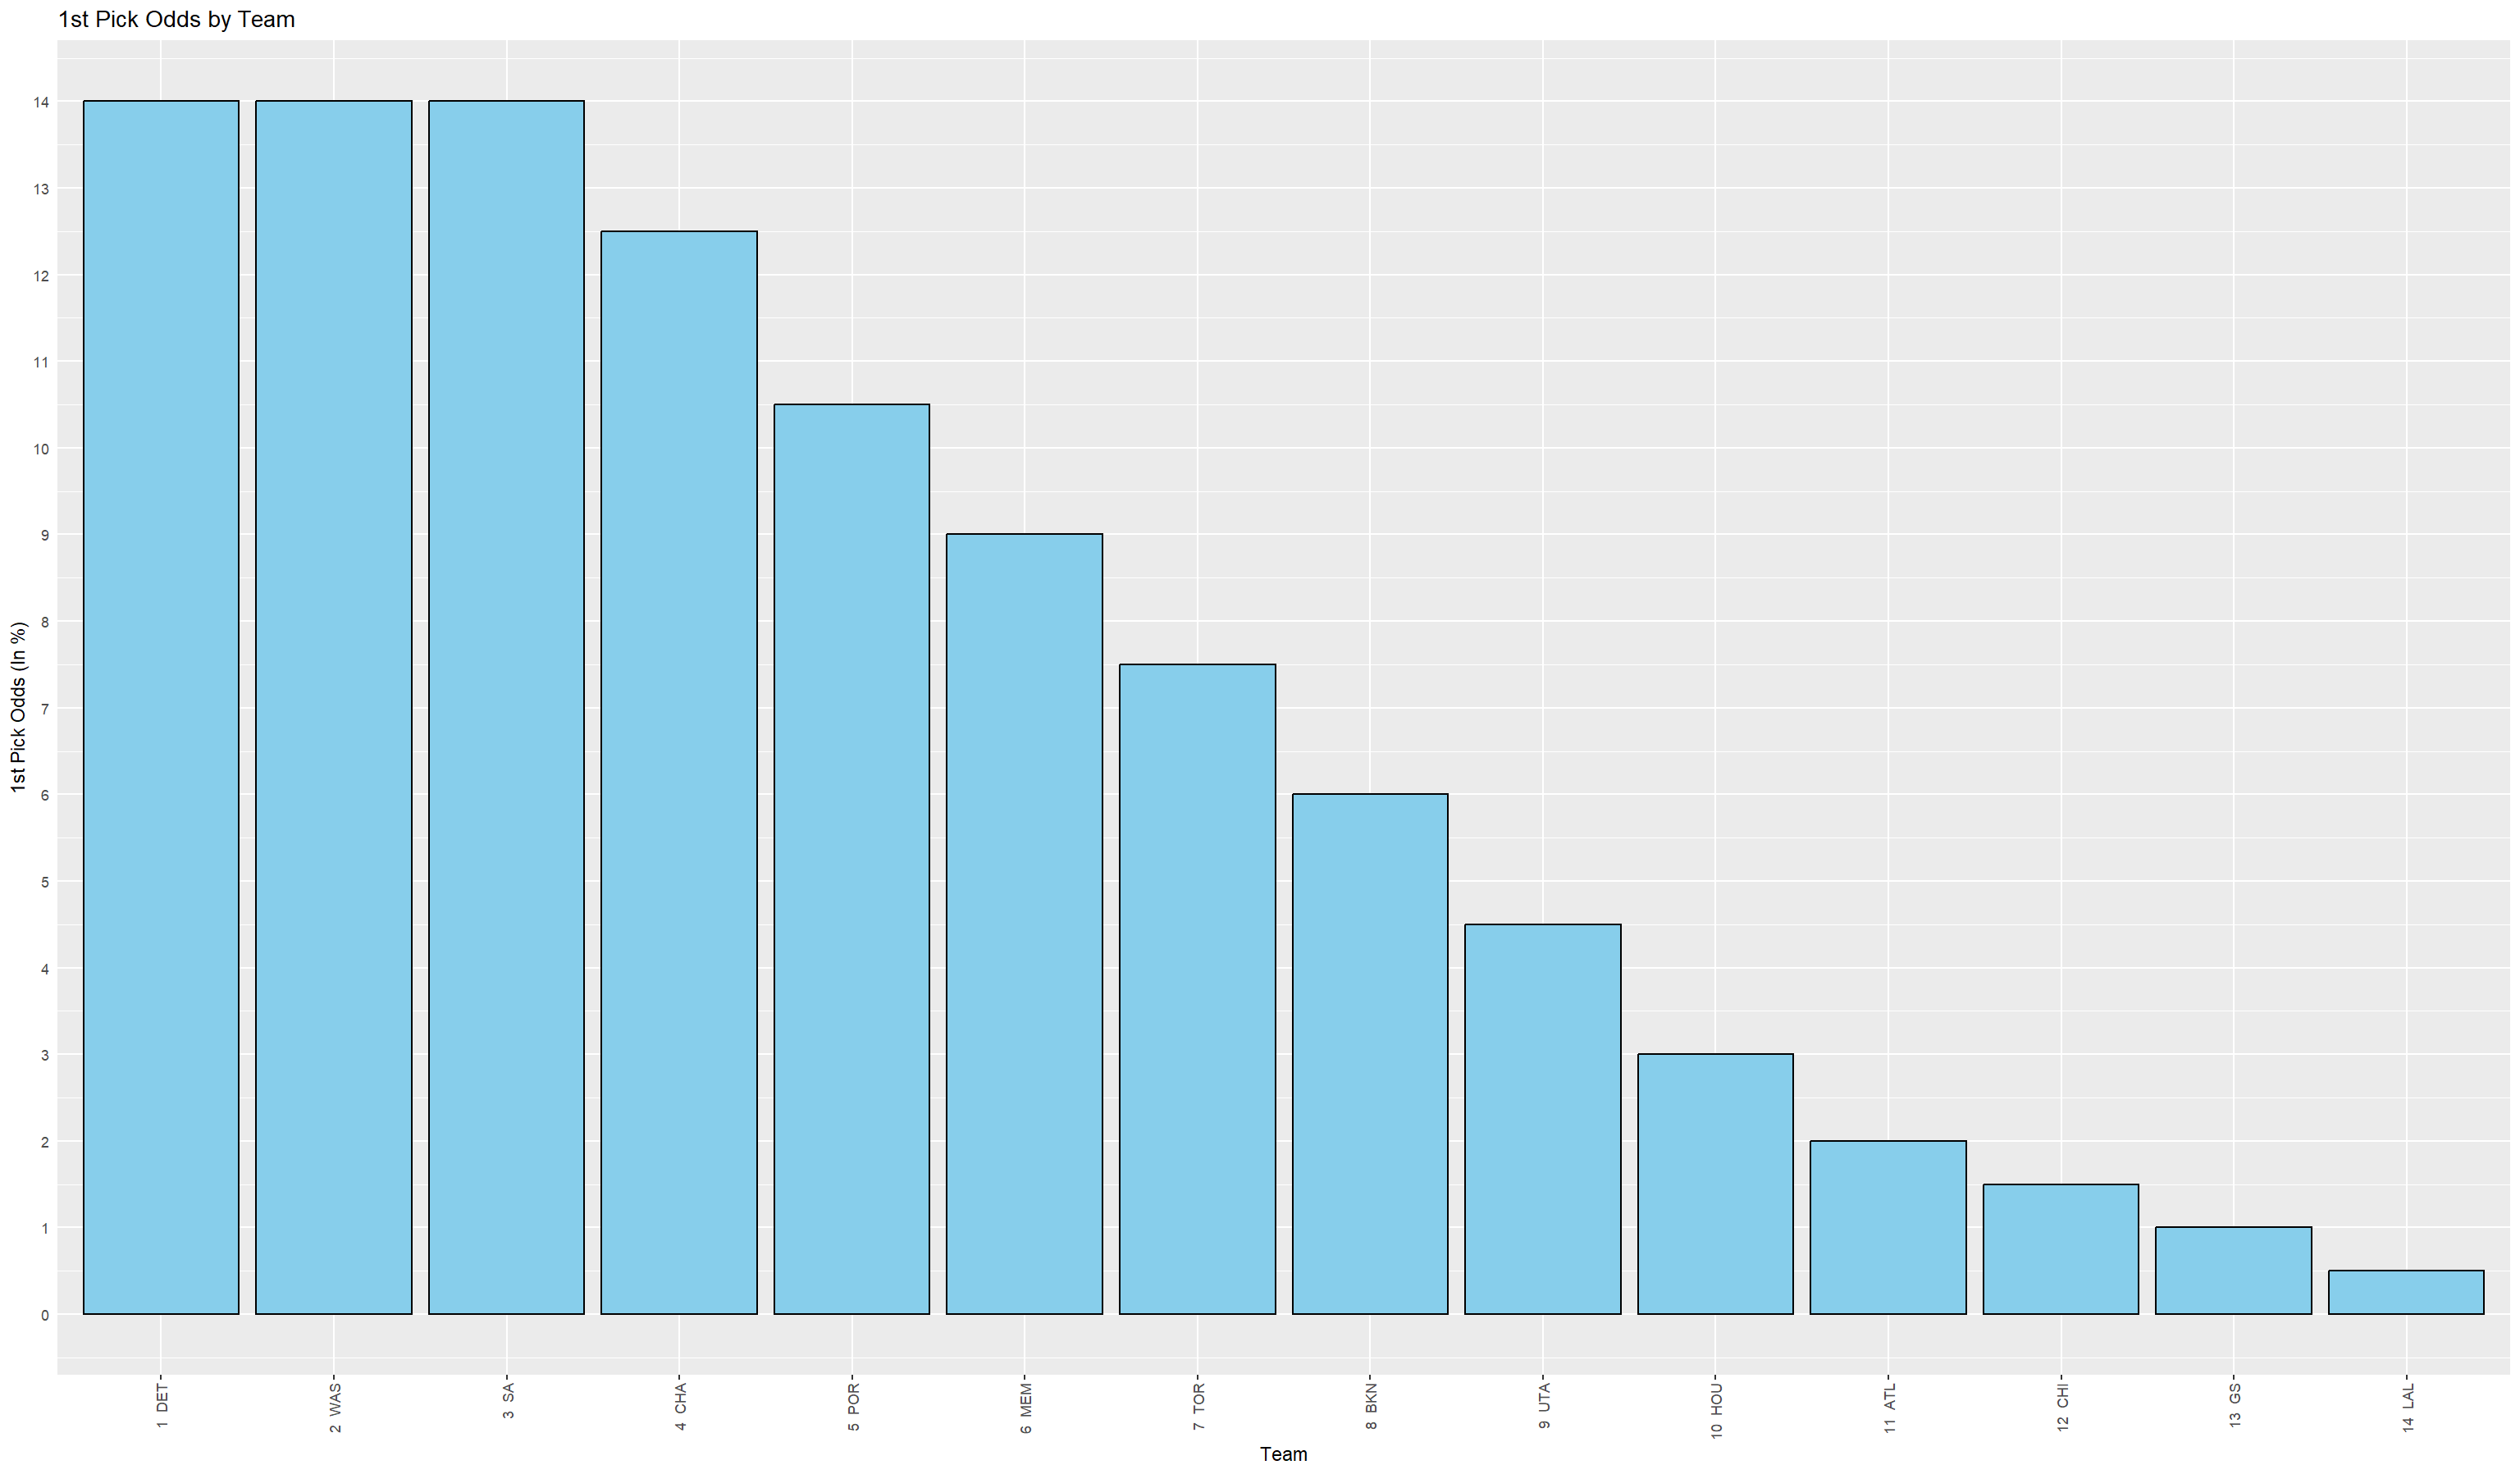
\includegraphics[width=0.5\linewidth]{PS6a_Thomasson.png}
    \caption{Who Gets the 1st Pick?}
    \label{fig:enter-label}
\end{figure}

My second plot is a distribution of the San Antonio Spurs' odds of their draft pick landing in each individual slot:

\begin{figure}
    \centering
    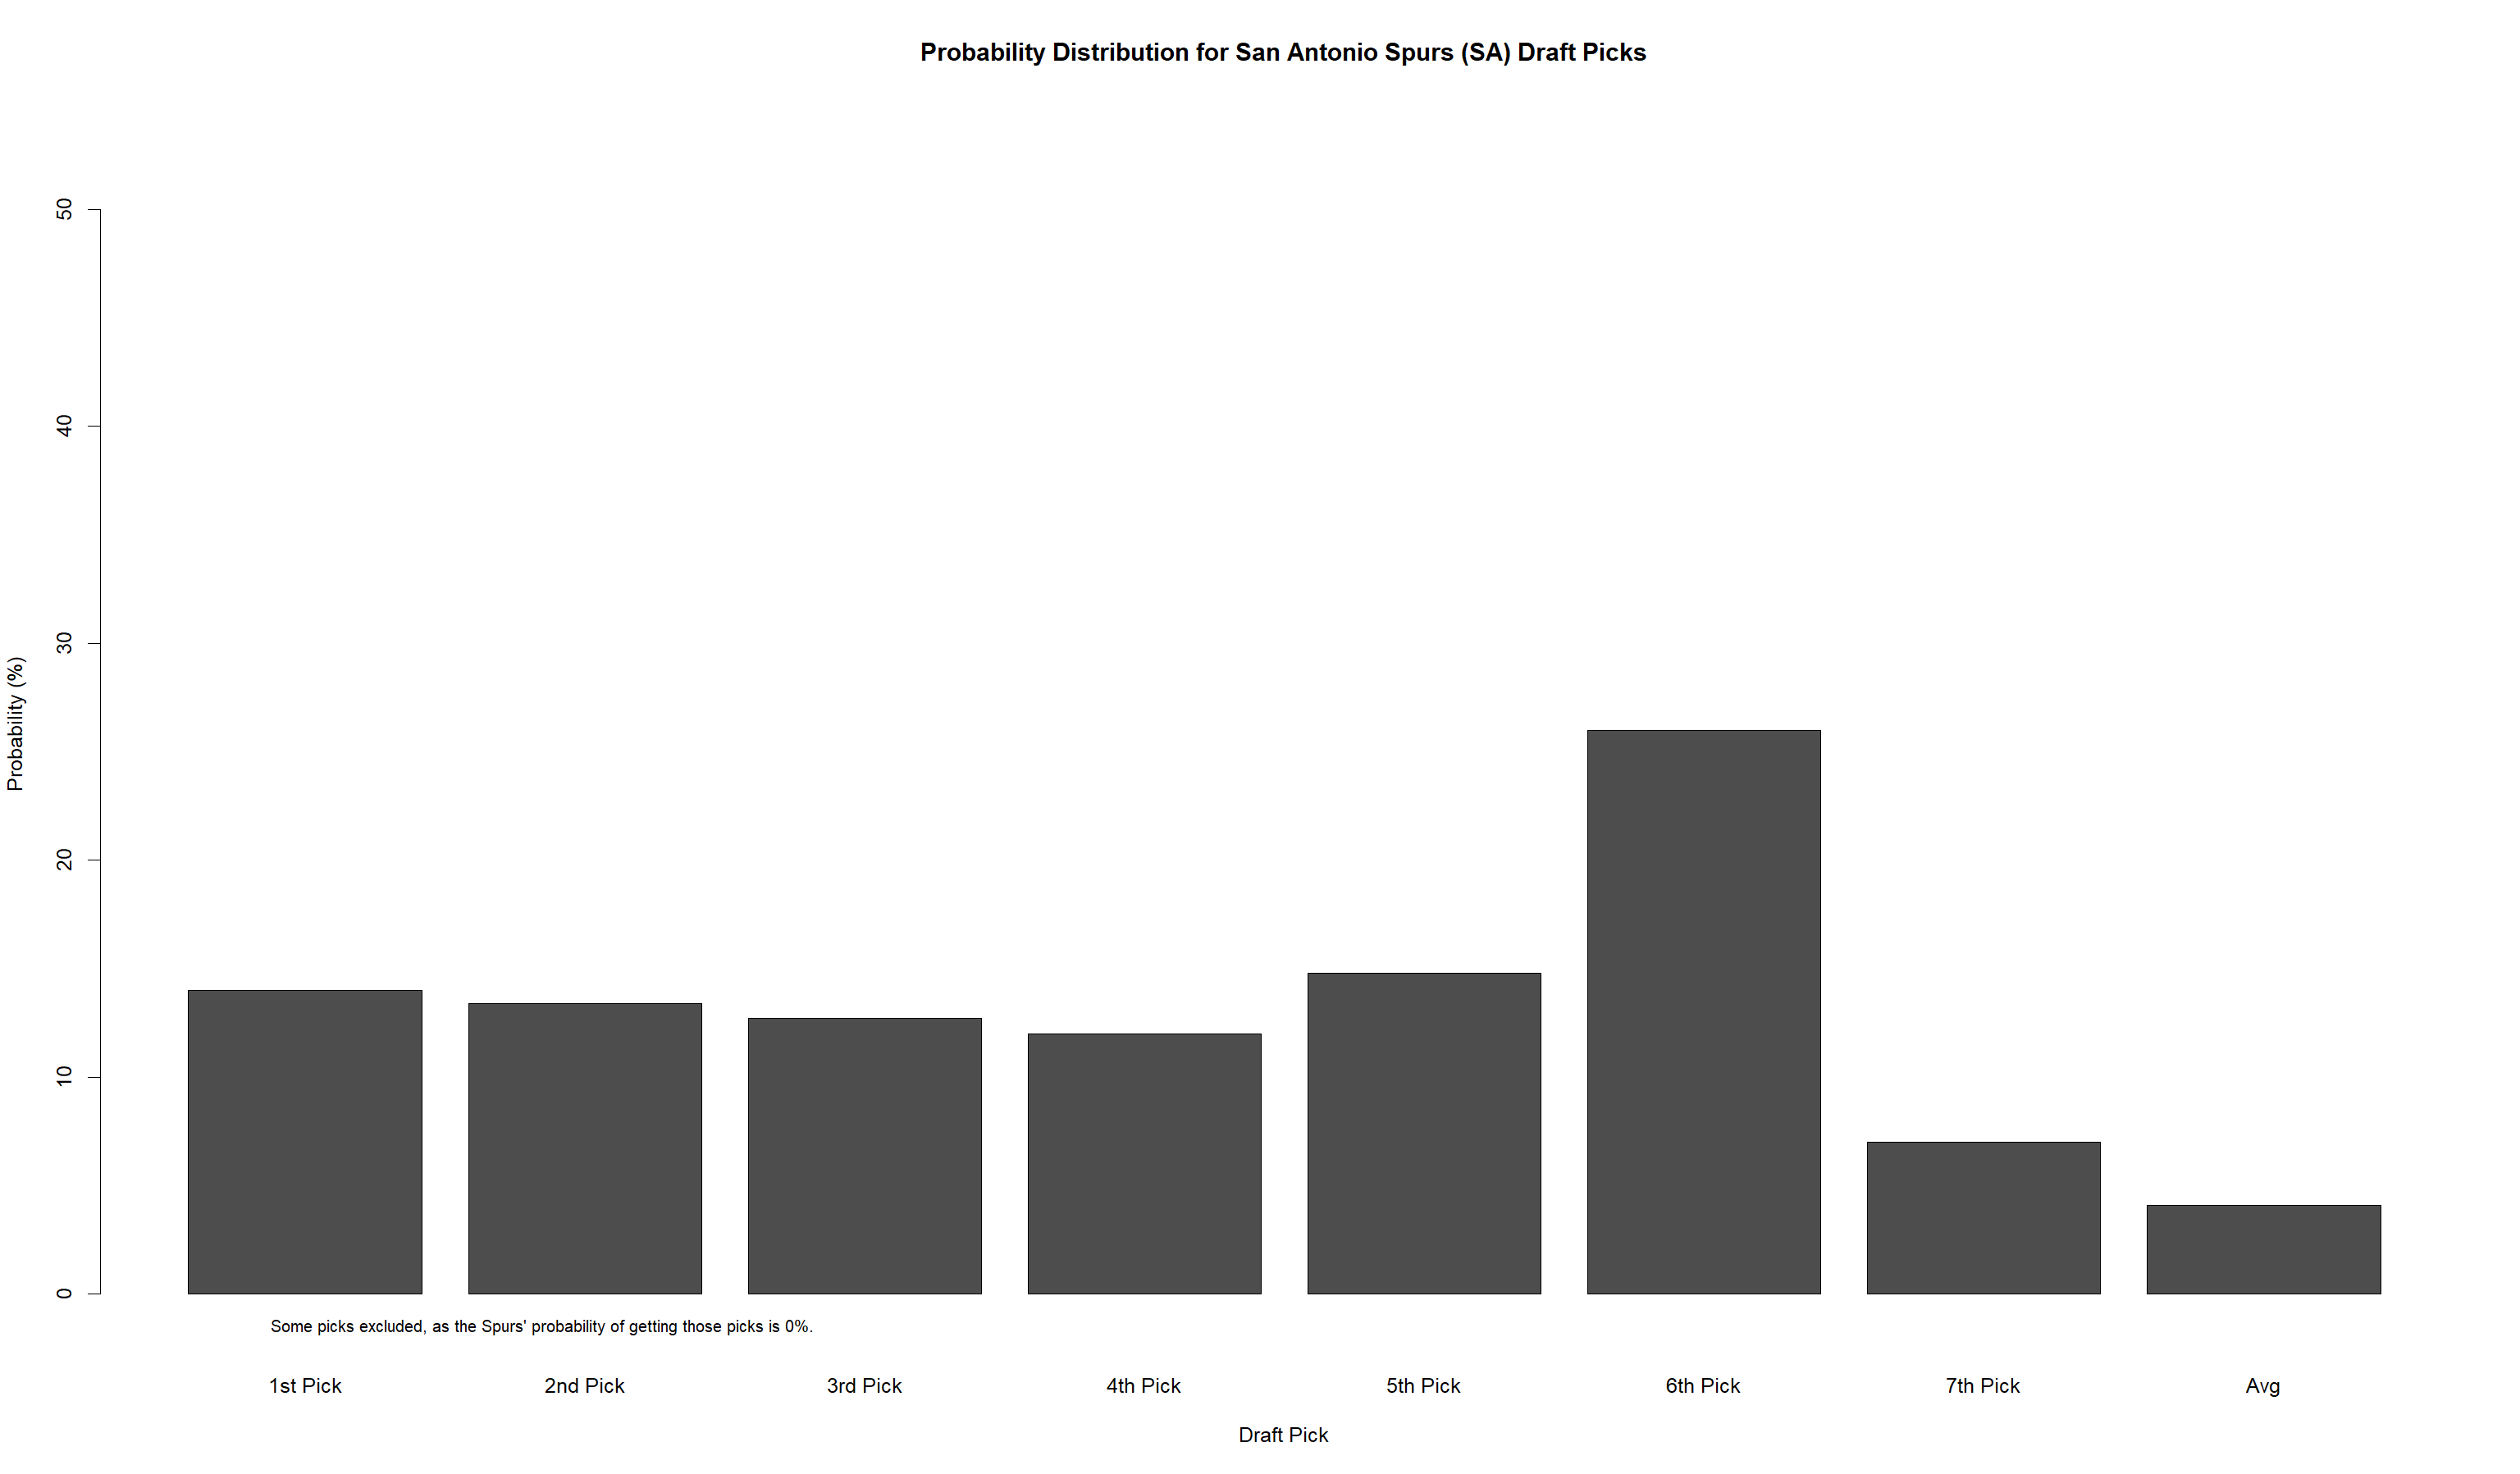
\includegraphics[width=0.5\linewidth]{PS6b_Thomasson.png}
    \caption{What Pick Do the Spurs Get?}
    \label{fig:enter-label}
\end{figure}

Finally, The Toronto Raptors have a Top-6 Protected Pick. If the pick lands outside of the Top 6, they lose the pick to the Spurs. I create a pie chart displaying the probability of "keeping" or "sending" the pick.

\begin{figure}
    \centering
    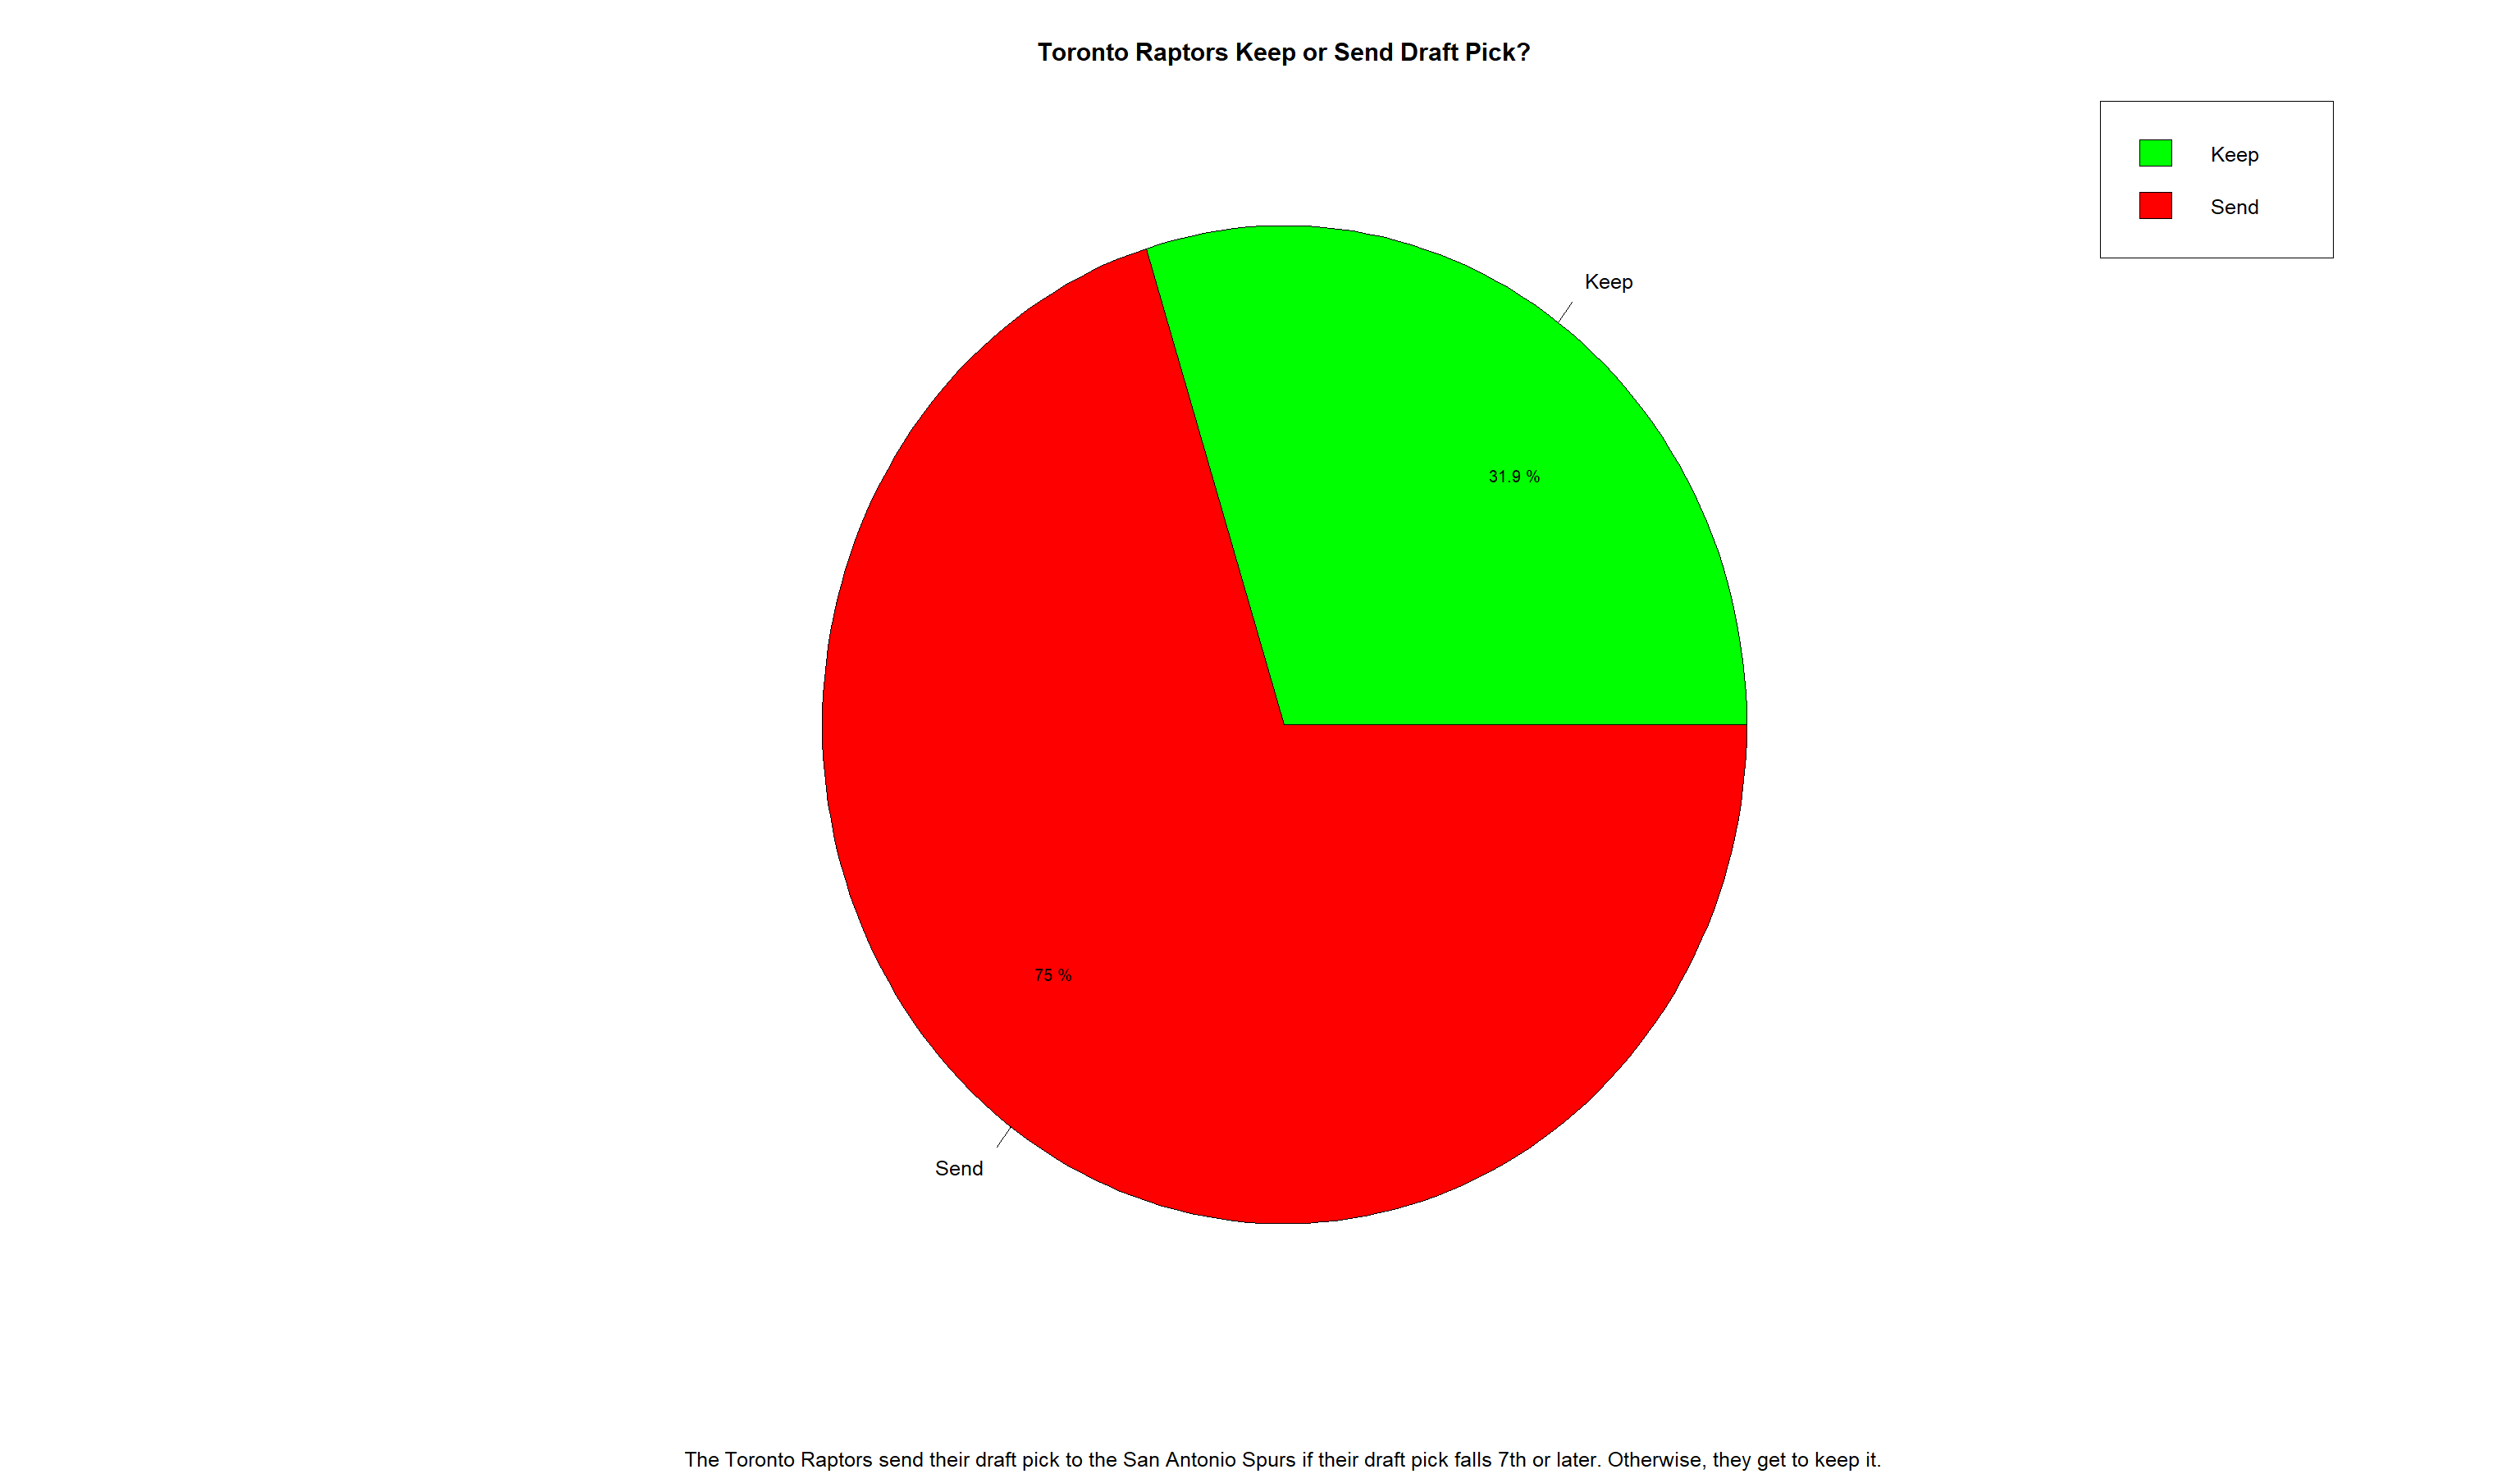
\includegraphics[width=0.5\linewidth]{PS6c_Thomasson.png}
    \caption{DO the Toronto Raptors Keep Their Pick?}
    \label{fig:enter-label}
\end{figure}

\end{document}